\chapter{Preemptive Multitasking}
\label{cha:preemptive_multitasking}

\section{Multiprocessor Support and Cooperative Multitasking}
\par 这一部分首先要向jOS扩展到一个多处理器的系统上,然后实现一些内核调用来允许用户级别的环境来创建新的环境。还需要实现轮训调度,在进程不使用CPU使允许内核切换到另一个进程。

\subsection{Multiprocessor Support}
\par 我们将使jOS支持对称多处理(SMP)系统。这种系统能够使所有的CPU对内存能和I/O够有相同的访问权限。虽然CPU在对称多处理的情况下以相同的方式工作,但是在启动过程中可以被分为2个类型:引导处理器(BSP)以及应用处理器(AP)。引导处理器用户初始化以及启动操作系统,而应用处理器被引导处理器启动。哪个处理器作为引导处理器由硬件决定。
\par 在对称多处理系统中,每个CPU都有一个本地APIC(LAIPC)单元。LAIPC单元用于传递中断并给它连接的CPU一个唯一的id。在这个lab中将使用LAIPC以下功能:
\begin{itemize}
    \item 从BSP读取LAPIC标识符来区分当前代码在那个CPU上运行。
    \item 从BSP发送STARTUP跨处理器中断到AP来启动其他CPU。
    \item 使用LAPIC的内置计时器编程来触发时钟中断以支持抢占式多任务处理。
\end{itemize}
\par 处理器通过应设在内存上的I/O(MMIO)来访问LAPIC。在MMIO中,物理内存的一部分被链接到I/O设备的寄存器。因此load/store指令可以用于访问设备的寄存器。LAPIC起始于物理地址0xfe000000。对于以前的直接到KERNBASE的映射来说这太高了。jOS在虚拟地址MMIOBASE留了4MB的空间,因此我们由空间来映射这一类的设备。

\exercise{1}{
    \par 实现kern/pmap.c中的mmio\_map\_region。查看kern/lapic.c来查看如何使用它。在对这一exercise进行测试之前需要先完成下一个exercise。
}
\begin{exerciseSolution}{1}
    \par 首先完成mmio\_map\_region。调用boot\_map\_region建立需要的映射。根据注释,需要注意使用的权限为PTE\_PCD|PCE\_PWT来防止CPU来cache这部分内存,此外还需要注意每次都需要更新base,以及超出内存的部分需要发出panic。
    \inputCodeSetLanguage{c}
    \begin{lstlisting}
void * mmio_map_region(physaddr_t pa, size_t size) {
    static uintptr_t base = MMIOBASE;

    if(base + ROUNDUP(size, PGSIZE) > MMIOLIM)
        panic("mmio_map_region: mmio overflow.");
    boot_map_region(kern_pgdir, base, ROUNDUP(size, PGSIZE), pa, PTE_W|PTE_PCD|PTE_PWT);
    uintptr_t temp = base;
    base += ROUNDUP(size, PGSIZE);
    return (void *)temp;
}
    \end{lstlisting}
\end{exerciseSolution}

\subsubsection{Application Processor Bootstrap}
\par 在启动AP之前,BSP理器首先需要收集处理器系统的信息,包括CPU总数,CPU的APIC id,LAPIC的MMIO地址。kern/mpconfig.c中的mp\_init()通过读取BIOS中的MP配置来获得这些信息。APs从实模式开始
\par boot\_aps函数启动了APs的引导。AP的音高过程类似于boot/boot.S中的bootloader启动过程。因此boot\_aps()将AP的入口复制到实模式可以访问的区域MPENTRY\_PADDR。然后boot\_aps()通过发送STARTUP跨处理器中断到LAPIC单元,逐个激活APs。激活时,首先初始化AP的CS:IP让其从入口执行代码,然后开启分页进入保护模式,然后调用mp\_main(),最后等待AP的CPU\_STARTED 信号,并开始激活下一个。

\exercise{2}{
    \par 阅读kern/init.c中的boot\_aps()以及mp\_main,以及kern/mpentry.S中的汇编。然后修改kern/pmap.c中的page\_init()实现,来避免将MPENTRY\_PADDR加入空闲链表,一次确保能够安全的复制AP的启动代码到这个物理地址并运行。代码应该能够通过更新过的check\_page\_free\_list测试。(但可能不会通过check\_kern\_pgdir测试)
}
\begin{exerciseSolution}{2}
    \par 将从MPENTRY\_PADDR开始的一个物理页标记为已使用,并能够将其加入链表。而MPENTRY\_PADDR=0x7000,在低地址处,因此将处理低地址的代码的循环中加入一个判断条件即可,即修改为如下代码:
    \inputCodeSetLanguage{c}
    \begin{lstlisting}
for (i = 1; i < npages_basemem; ++i) {
    if(i == MPENTRY_PADDR/PGSIZE){
        pages[i].pp_ref = 1;
        continue;
    }
    pages[i].pp_ref = 0;
    pages[i].pp_link = page_free_list;
    page_free_list = &pages[i];
}
    \end{lstlisting}
    \par 修改完成后重新编译并运行qemu,其显示输出如图\ref{fig:lab4/exercise2_1}所示。
    \begin{figure}[htb]
        \centering
        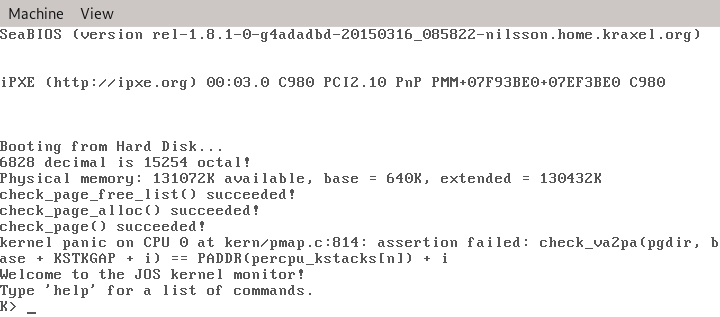
\includegraphics[width=0.8\linewidth]{lab4/exercise2_1.png}
        \caption{通过check\_page\_free\_list测试}
        \label{fig:lab4/exercise2_1}
    \end{figure}
\end{exerciseSolution}

\begin{questionEnv}
    \begin{enumerate}
        \item 比较kern/mpentry.S以及boot/boot.S。记住kern/mpentry.S的目标是向内核一样在KERNBASE之上运行。宏MPBOOTPHYS的作用是什么?为什么在kern/mpentry.S中它是必要的但是boot/boot.S中它不是必要的?也就是说,如果kern/mpentry.S中不写MPBOOTPHYS会发生什么?
    \end{enumerate}
\end{questionEnv}
\begin{answer}
    \begin{enumerate}
        \item 根据MPBOOTPHYS的内容可知,起作用是将高地址转换为绝对地址址。因为此时还出于实模式,但是代码中的地址为高地址,因此需要进行转换。
    \end{enumerate}
\end{answer}

\subsubsection{Per-CPU State and Initialization}
\par 在写一个多处理器操作系统时,区分CPU的私有状态以及全局状态非常关键。kern/cpu.h定义了大部分的私有状态。应该注意的私有状态有:
\begin{itemize}
    \item Per-CPU 内核栈。
        \par 多个CPU可能同时陷入内核状态,因此需要给每个处理器一个独立于其他CPU的的内核栈。数组percpu\_kstacks[NCPU][KSTKSIZE]为NCPU个内核栈保留了空间。在Lab2中BSP的内核栈映射到了KSTACKTOP下方,而在lab4中需要把每个CPU的内核栈都映射到这个区域。每个栈之间留下一个空也作为缓冲区避免溢出。
    \item Per-CPU TSS和TSS描述符
        \par 为了标识每个CPU内核栈的位置,需要任务状态段(TSS)
    \item Per-CPU 当前环境指针
        \par 每个CPU能够同时运行各自的用户进程因此重新定义了curenv。
    \item Per-CPU 系统寄存器
        \par 所有的寄存器包括系统寄存器都是CPU私有的,因此初始化寄存器的指令需要在每个CPU执行一次。
\end{itemize}
\exercise{3}{
    \par 修改kern/pmap.c中的mem\_init\_mp()来映射开始于KSTACKTOP的per-CPU内核栈。每个栈的大小是KSTKSIZE加上KSTKGAP字节的不被映射的空间。代码应该能够通过新的check\_kern\_pgdir()测试。
}
\begin{exerciseSolution}{3}
    \par 在这一部分代码中,只需要像lab2一样逐个映射每一个栈的内存地址即可。在这一部分中,虽然BSP的栈地址之前已经映射过,但是更换物理地址不会增删页面引用,因此不修改之前的引用也不会出现问题。
    \inputCodeSetLanguage{c}
    \begin{lstlisting}
static void mem_init_mp(void) {
    uint32_t i;
    uintptr_t start = KSTACKTOP-KSTKSIZE;
    for(i=0; i < NCPU; ++i){
        boot_map_region(kern_pgdir, (uintptr_t)(start), KSTKSIZE, PADDR(percpu_kstacks[i]), PTE_W);
        start -= (KSTKSIZE + KSTKGAP);
    }
}
    \end{lstlisting}
    \par 补完这一部分代码后重新编译运行qemu,结果如图\ref{fig:lab4/exercise3_1}所示,能够成功通过check\_kern\_pgdir()测试。
    \begin{figure}[htb]
        \centering
        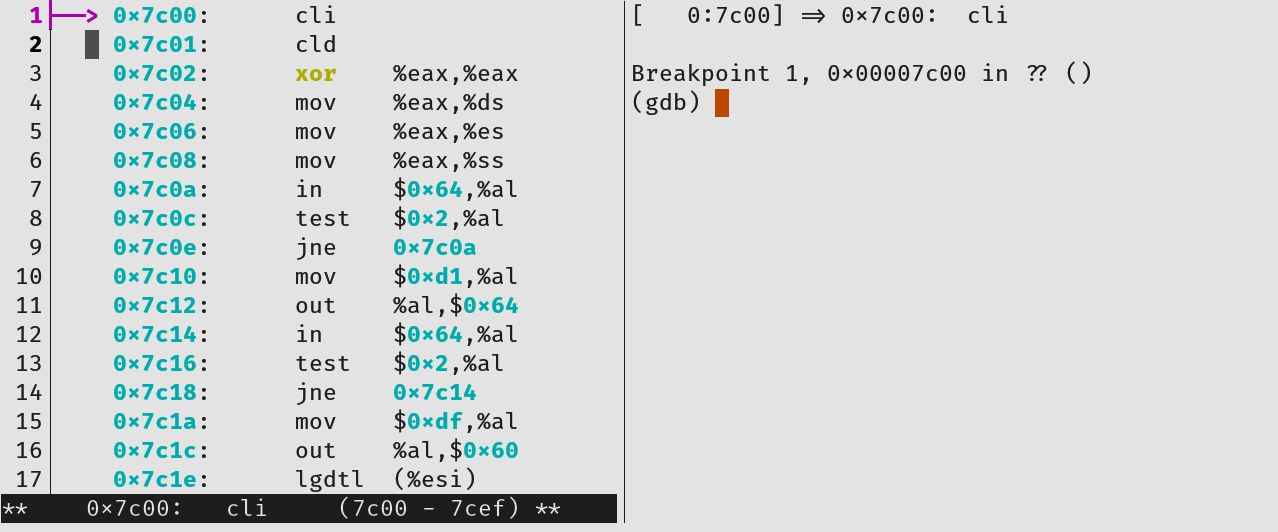
\includegraphics[width=0.7\linewidth]{lab4/exercise3_1.png}
        \caption{通过check\_kern\_pgdir测试}
        \label{fig:lab4/exercise3_1}
    \end{figure}
    \FloatBarrier
\end{exerciseSolution}

\exercise{4}{
    \par kern/trap.c中的trap\_init\_percpu()代码为了BSP初始化TSS以及TSS描述符。在Lab3中它是工作正确的,但是在运行其他CPU是运行不正确。修改这部分代码使它能在所有CPU上运行。
}
\begin{exerciseSolution}{4}
    \par 根据注释中的提示我们可以知道thiscpu总是指向当前cpu的信息,而第i个CPU的TSS描述符为$gdt[(GD\_TSS0 >> 3) + i]$,再参考用于初始化BSP的代码,修改后的代码如下:
    \inputCodeSetLanguage{c}
    \begin{lstlisting},
void trap_init_percpu(void) {
    struct Taskstate *thists = &thiscpu->cpu_ts;

    thists->ts_esp0 = KSTACKTOP - thiscpu->cpu_id * (KSTKSIZE + KSTKGAP);
    thists->ts_ss0 = GD_KD;
    thists->ts_iomb = sizeof(struct Taskstate);

    gdt[(GD_TSS0 >> 3) + thiscpu->cpu_id] =
        SEG16(STS_T32A, (uint32_t) (thists), sizeof(struct Taskstate) - 1, 0);
    gdt[(GD_TSS0 >> 3) + thiscpu->cpu_id].sd_s = 0;

    ltr(GD_TSS0 + (thiscpu->cpu_id << 3));
    lidt(&idt_pd);
}
    \end{lstlisting}
    \par 修改完成后按照指导输入make qemu CPUS=4,输出结果如图\ref{fig:lab4/exercise4_1}所示。说明
    \begin{figure}[htb]
        \centering
        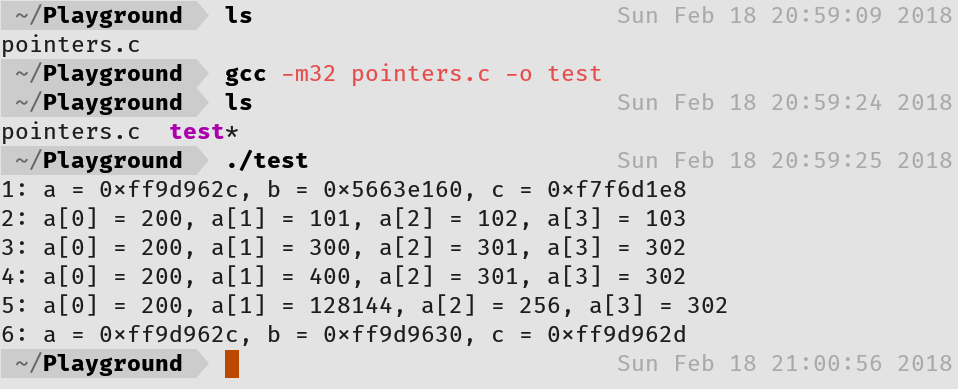
\includegraphics[width=0.8\linewidth]{lab4/exercise4_1.png}
        \caption{使用CPUS=4启动qemu界面}
        \label{fig:lab4/exercise4_1}
    \end{figure}
\end{exerciseSolution}

\subsubsection{Locking}
\par 当前代码在初始化AP之后就会开始自旋,在让AP进一步执行之前,首先需要解决多个CPU运行内核的地址竞态。最简单的方法是使用big kernel lock,也就是使用一个全局的锁来锁住整个内核,并在环境返回用户模式时释放这个锁。此时用户环境可以运行在多个CPU上但是内核只能运行在一个CPU上。
\par kern/spinlock.h声明了这个big kernel lock,名称为kernel\_lock。它也提供了lock\_kernel以及unlock\_kernel来加锁和解锁。在以下四个地方应该加锁:
\begin{itemize}
    \item i386\_init()中,BSP唤醒其他CPU之前。
    \item mp\_main()中,在初始化AP之后加锁,并调用sched\_yield来在这个AP上运行用户环境。
    \item 在trap()中,从用户模式进入内核模式需要加锁。检查tf\_cs的较低比特来判断当前是在用户环境中还是在内核中。
    \item 在env\_run()中,在切换到用户模式前解锁。不要太晚或太早解锁,否则可能产生死锁或竞态。
\end{itemize}

\exercise{5}{
    \par 按照上述描述使用big kernel lock。使用lock\_kernel()以及unlock\_kernel()在适当的地方加锁和解锁。
}
\begin{exerciseSolution}{5}
    \par 按照提示在这一节所描述的3个地方(i386\_init, mp\_main以及trap中)加锁即可。注意的是unlock\_kernel()应该置于env\_pop\_tf(\&curenv->env\_tf);之前而不是其他位置。重新编译并运行代码可以发现exercise4中出现的kernel panic消失了,但也由于锁的原因并没有进入user mode。如图\ref{fig:lab4/exercise5_1}所示。
    \begin{figure}[htb]
        \centering
        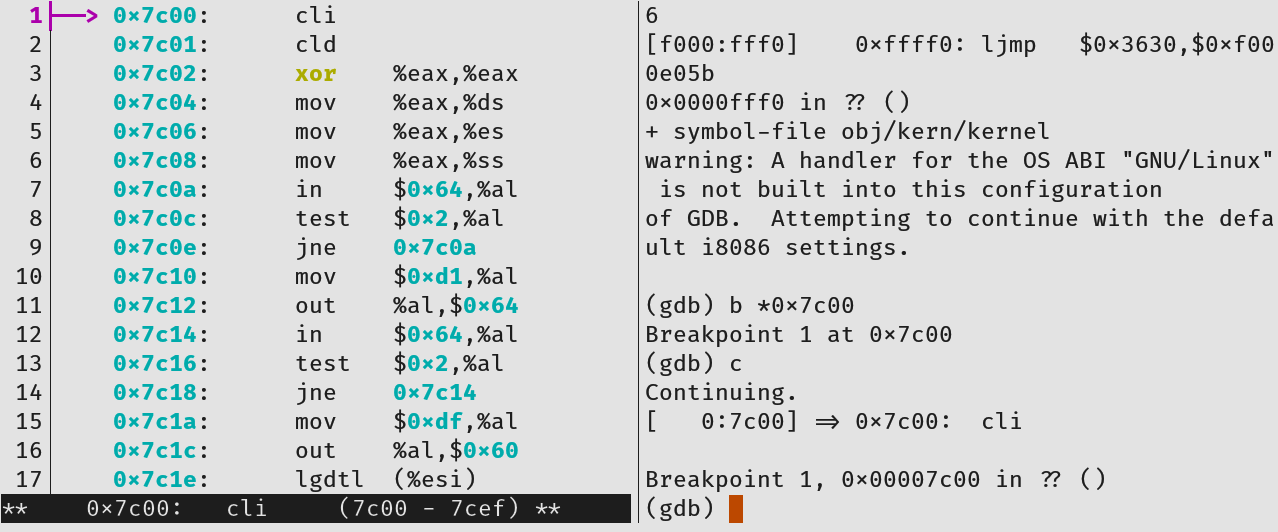
\includegraphics[width=0.8\linewidth]{lab4/exercise5_1.png}
        \caption{加上big kernel lock后运行qemu结果}
        \label{fig:lab4/exercise5_1}
    \end{figure}
\end{exerciseSolution}

\begin{questionEnv}
    \begin{enumerate}
        \setcounter{enumi}{1}
    \item 看来使用大内核锁能够保证一次只有一个CPU能够运行内核代码。为什么我们还是需要为每个CPU准备一个不同的内核栈呢?使用``即使加上了big kernel lock,共享内核栈依然会出错''来描述原因。
    \end{enumerate}
\end{questionEnv}
\begin{answer}
    \begin{enumerate}
        \setcounter{enumi}{1}
    \item 因为在进入内核之前也可能对内核栈进行了操作,例如trap之前向内核中压入寄存器信息等。
    \end{enumerate}
\end{answer}

\subsection{Round-Robin Scheduling}
\par 这一节的任务是修改内核使之能够进行轮询调度。轮训调度按照如下规则工作:
\begin{itemize}
    \item kern/shed.c中的sched\_yield函数负责选择一个新的环境运行。它按圈顺序搜索envs[]数组(如果之前没有运行的环境则选择数组的开头),选择第一个有ENV\_RUNNABLE状态的环境,并调用env\_run()跳转到那个环境中。
    \item sched\_yield()不能同时在两个CPU上运行同一个环境。如果环境已经在某一个CPU上运行,则其状态会变为ENV\_RUNNING。
    \item 程序中已经实现了一个新的系统调动sys\_yield(),用户进程可以调用它来放弃CPU使用权限。
\end{itemize}

\begin{exerciseEnv}{6}
    \par 在sched\_yield()中实现一个轮询式调度,并修改syscall()来分发sys\_yield()。
    \par 确保在mp\_main()中调用了sched\_yield()。
    \par 修改kern/init.c来创建三个或更多的环境来运行用户程序user/yield.c
    \par 运行make qemu,应该能看到环境在结束前来回切换5次,输出如下。
    \par 使用多个CPU进行测试:make qemu CPUS=2
    \inputCodeSetLanguage{bash}
    \begin{lstlisting}[numbers=none]
...
Hello, I am environment 00001000.
Hello, I am environment 00001001.
Hello, I am environment 00001002.
Back in environment 00001000, iteration 0.
Back in environment 00001001, iteration 0.
Back in environment 00001002, iteration 0.
Back in environment 00001000, iteration 1.
Back in environment 00001001, iteration 1.
Back in environment 00001002, iteration 1.
...
    \end{lstlisting}
    \par 在yield程序退出后,将会没有可运行的环境。调度器应该调用jOS kernel monitor。如果没有发生则表明需要修改代码。
\end{exerciseEnv}
\begin{exerciseSolution}{6}
    \par 首先在kern/sched.c中实现轮询调度,按照题目描述使用按圈轮询的方式,实现的调度代码如下
    \inputCodeSetLanguage{c}
    \begin{lstlisting}
void sched_yield(void) {
    int counter;
    if (curenv) {
        for (counter = ENVX(curenv->env_id) + 1;
                counter != ENVX(curenv->env_id);
                counter = (counter + 1) % NENV)
            if (envs[counter].env_status == ENV_RUNNABLE)
                env_run(envs + counter);
    } else {
        for (counter = 0; counter < NENV; ++counter)
            if (envs[counter].env_status == ENV_RUNNABLE)
                env_run(envs + counter);
    }

    // sched_halt never returns
    sched_halt();
}
    \end{lstlisting}

    \par 然后,在syscall中添加一个case来使用sys\_yield系统调用:
    \begin{lstlisting}
case SYS_yield:
    sys_yield();
    return 0;
    \end{lstlisting}

    \par 最后,修改kern/init.c中的用户进程。在sched\_yield();前添加:
    \begin{lstlisting}
    ENV_CREATE(user_yield, ENV_TYPE_USER);
    ENV_CREATE(user_yield, ENV_TYPE_USER);
    ENV_CREATE(user_yield, ENV_TYPE_USER);
    \end{lstlisting}

    \par 修改完成后,重新编译,运行make qemu CPUS=2,结果如图\ref{fig:lab4/exercise6_1},程序切换5次后退出,与预想的一致。
    \begin{figure}[htb]
        \centering
        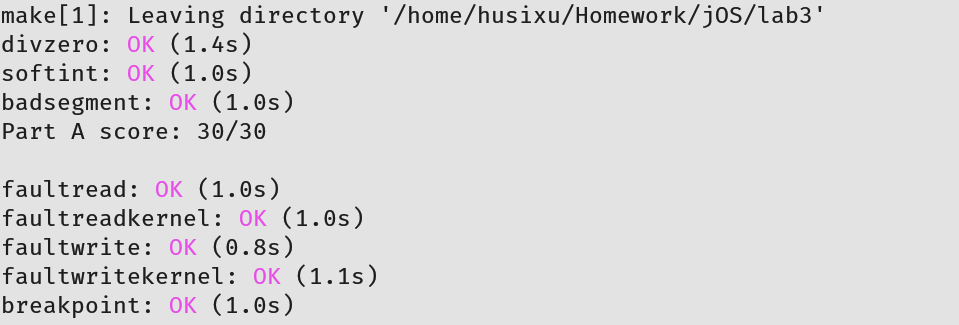
\includegraphics[width=0.8\linewidth]{lab4/exercise6_1.png}
        \caption{运行3份user/yield的输出}
        \label{fig:lab4/exercise6_1}
    \end{figure}
\end{exerciseSolution}

\begin{questionEnv}
    \begin{enumerate}
        \setcounter{enumi}{2}
        \item 在的env\_run实现中应该调用了lcr3()。在调用lcr3之前和之后代码进行了对于变量env\_run的参数e的引用。在加载\%cr3寄存器时,MMU使用的地址环境被改变了。但是虚拟地址的意义与给定的地址上下文有关联:地址上下文指定了虚拟地址映射到的物理地址。那么指针为什么在地址切换前后都能够正常解引用?
        \item 任何时候,如果内核从一个环境切换到了另一个,它必须保证老的内核环境寄存器被保存了,以保证她们能够被正确的还原。为什么?这在那里发生的?
    \end{enumerate}
\end{questionEnv}

\begin{answer}
    \begin{enumerate}
        \setcounter{enumi}{2}
        \item 在lab3中env\_setup\_vm以内核的页目录作为模板初始化了用户环境。因此两个环境的e映射到了同一个物理地址,因此才能够正确的解引用。
        \item 保存在kern/trapentry.S中的\_alltraps处,而恢复发生在kern/env.c中的env\_pop\_tf处。只有保证内核调用前后栈的内容没有变化才能使用户程序继续正确执行。
    \end{enumerate}
\end{answer}

\subsection{System Calls for Environment Creation}
\par 虽然内核可以运行并切换多个用户环境了,但是现在只能运行内核设置好的程序。现在需要实现一个新的系统调用,以允许用户创建并开始新的用户环境。
\par Unix提供了fork系统调用来创建进程,它会复制父进程的地址空间来创建子进程。唯一的区别是进程ID。在父进程中,fork返回子进程的id,而在子进程中返回0。父子进程的地址空间是独立的。
\par 现在需要创建一个更原始的jOS系统调用来创建一个用户环境。在这个系统调用中需要实现一个类Unix的fork()。加上一些其他的用户环境创建。新的jOS系统调用如下:
\begin{itemize}
    \item sys\_exofork:
        \par 这个系统调用创建一个空白进程,在其用户空间中不映射物理内存,并且它是不可运行的。在刚开始它会和父进程有相同的寄存器状态。sys\_exofork还会返回子进程的envid\_t,子进程返回0。
    \item sys\_env\_set\_status:
        \par 设置指定进程的状态为ENV\_RUNNABLE或者ENV\_NOT\_RUNNABLE。这个系统调用通常用来标记在地址空间和寄存器状态被初始化之后的新环境就绪。
    \item sys\_page\_alloc:
        \par 分配物理地址空间并将其映射到用户环境空间的虚拟地址。
    \item sys\_page\_map:
        \par 复制一个用户环境的页映射到另一个用户环境,也就是共享内存。
    \item sys\_page\_unmap:
        \par 删除用户环境的虚拟内存映射。
\end{itemize}
\par 对于所有接收环境id的系统调用,jOS内核支持从值0到``当前用户环境''的转换。这个转换被envid2env实现。

\exercise{7}{
    \par 在kern/syscall.c实现上述系统调用。
    \par 实现kern/syscall.c中的上述系统调用。你需要kern/pmap.c以及kern/env.c中的不同函数,尤其是envid2env。现在无论在什么时候调用envid2env,都需要传递一个checkperm参数。使用user/dumbfork来测试内核。
}
\begin{exerciseSolution}{7}
    \par 首先实现sys\_exofork函数,该函数分配一个新的进程但是不做内存复制处理。其关键是如何处理父进程返回子进程id而子进程返回0的问题。于是子进程复制父进程的TrapFrame并将TrapFrame中eax的值设置为0,而函数本身返回子进程的id。这样在运行env\_run时就可以获得不同的返回值了。最后实现的代码如下:
    \inputCodeSetLanguage{c}
    \begin{lstlisting}
static envid_t sys_exofork(void) {
    struct Env *environment;
    int res;
    if((res = env_alloc(&environment, curenv->env_id)) < 0)
        return res;
    environment->env_status = ENV_NOT_RUNNABLE;
    environment->env_tf = curenv->env_tf;
    environment->env_tf.tf_regs.reg_eax = 0;
    return environment->env_id;
}
    \end{lstlisting}

    \par 然后是sys\_page\_alloc函数,该函数在环境的目标地址va分配一个页面并设置权限为perm。在实现这个函数时,首先需要检查目标地址以及权限是否合法。根据注释提示,如果page\_insert失败了还需要释放页面。
    \begin{lstlisting}
static int sys_page_alloc(envid_t envid, void *va, int perm) {
    if(!(perm & PTE_U) || !(perm & PTE_U) ||
            (perm & (~PTE_SYSCALL)) ||
            va > (void *)UTOP ||
            va != ROUNDDOWN(va, PGSIZE))
        return -E_INVAL;
    struct PageInfo *pginfo = page_alloc(ALLOC_ZERO);
    if(!pginfo)
        return -E_NO_MEM;
    struct Env *environment;
    if(envid2env(envid, &environment, 1) < 0)
        return -E_BAD_ENV;
    if(page_insert(environment->env_pgdir, pginfo, va, perm) < 0){
        page_free(pginfo);
        return -E_NO_MEM;
    }
    return 0;
}
    \end{lstlisting}
    \par 接下来是sys\_page\_map函数。简单的来说,这个函数就是建立跨进程的映射。较为重要的是根据注释对于参数逐个进行检查以及建立正确的映射。
    \begin{lstlisting}
static int
sys_page_map(envid_t srcenvid, void *srcva,
         envid_t dstenvid, void *dstva, int perm) {
    if((uint32_t)srcva >= UTOP || PGOFF(srcva) ||
            (uint32_t)dstva >= UTOP || PGOFF(dstva) ||
            !(perm & PTE_U) || !(perm & PTE_U) ||
            (perm & (~PTE_SYSCALL)) )
        return -E_INVAL;
    struct Env *src_environemt, *dst_environment;
    if(envid2env(srcenvid, &src_environemt, 1) < 0 ||
            envid2env(dstenvid, &dst_environment, 1) < 0)
        return -E_BAD_ENV;
    pte_t *pte;
    struct PageInfo *page = page_lookup(src_environemt->env_pgdir, srcva, &pte);
    if(!page || (!(*pte & PTE_W) && (perm & PTE_W)))
        return -E_INVAL;
    if(page_insert(dst_environment->env_pgdir, page, dstva, perm) < 0)
        return -E_NO_MEM;
    return 0;
}
    \end{lstlisting}

    \par 然后是sys\_page\_unmap函数,用于取消sys\_page\_map建立的映射。

    \begin{lstlisting}
sys_page_unmap(envid_t envid, void *va) {
    if((uint32_t)va >= UTOP || PGOFF(va))
        return -E_INVAL;
    struct Env *environment;
    if(envid2env(envid, &environment, 1) < 0)
        return -E_BAD_ENV;
    page_remove(environment->env_pgdir, va);
    return 0;
}
    \end{lstlisting}

    \par 然后实现sys\_env\_set\_status函数,在子进程内存映射结束后设置状态。与上面几个函数相同,需要注意的是对于参数的检查。
    \begin{lstlisting}
static int
sys_env_set_status(envid_t envid, int status) {
    if(status != ENV_RUNNABLE && status != ENV_NOT_RUNNABLE)
        return -E_INVAL;
    struct Env *environment;
    if(envid2env(envid, &environment, 1) < 0)
        return -E_BAD_ENV;
    environment->env_status = status;
    return 0;
}
    \end{lstlisting}

    \par 最后,需要在syscall函数中添加新的系统调用的分发,否则不能正常执行这些系统调用,即在switch中添加如下几行:
    \begin{lstlisting}
case SYS_exofork:
    return sys_exofork();
case SYS_env_set_status:
    return sys_env_set_status(a1, a2);
case SYS_page_alloc:
    return sys_page_alloc(a1, (void *) a2, a3);
case SYS_page_map:
    return sys_page_map(a1, (void *) a2, a3, (void *) a4, a5);
case SYS_page_unmap:
    return sys_page_unmap(a1, (void *) a2);
    \end{lstlisting}

    \par 运行make run-dumbfork,输出如图\ref{fig:lab4/exercise7_1}所示。父进程在10次迭代以后退出,而子进程在20次迭代以后退出。
    \begin{figure}[htb]
        \centering
        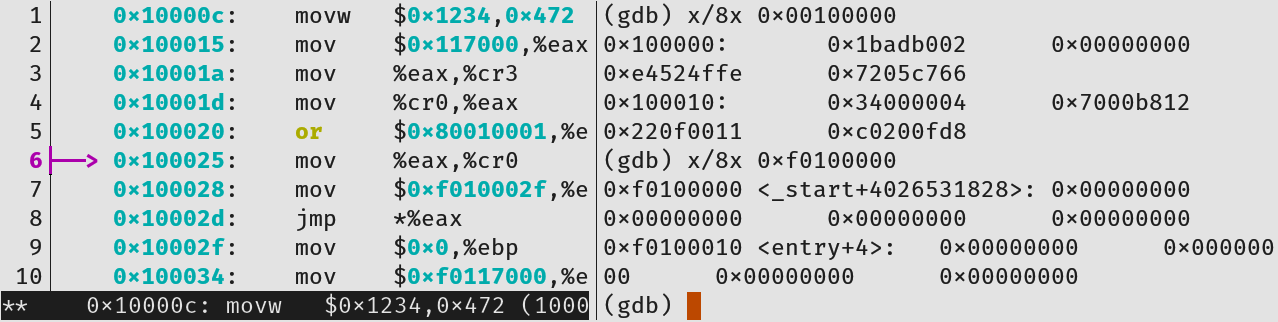
\includegraphics[width=0.6\linewidth]{lab4/exercise7_1.png}
        \caption{运行make run-dumbfork结果}
        \label{fig:lab4/exercise7_1}
    \end{figure}
    \FloatBarrier
\end{exerciseSolution}
\par 至此第一部分结束,运行make grade以后第一部分能够正常通过,如图\ref{fig:lab4/exercise7_2}所示。
\begin{figure}[htb]
    \centering
    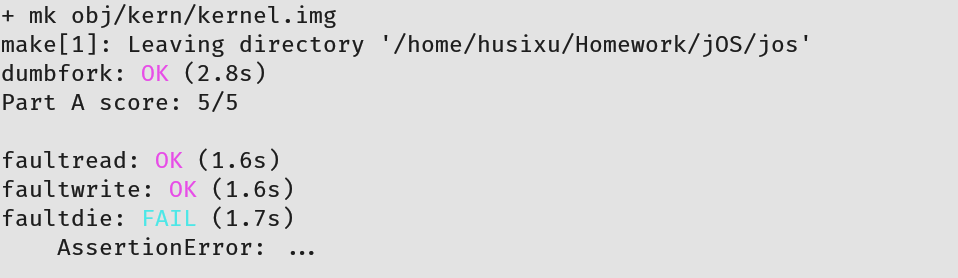
\includegraphics[width=0.8\linewidth]{lab4/exercise7_2.png}
    \caption{运行make grade的部分结果}
    \label{fig:lab4/exercise7_2}
\end{figure}

\section{Copy-on-Write Fork}
\par Part A中实现的类Unix系统调用较为原始。xv6将父进程的页复制新的进程页来创建子进程。而这个复制的过程则是整个fork最为昂贵的操作。然而调用了fork之后子进程通常会调用exec()将子进程的内存更换为新的程序,在这种情况下复制父进程的内存这个操作就被浪费了。
\par 因此后来的Unix系统让父子进程桐乡同一片物理区域,直到某个进程修改了内存。这个技术叫做copy-on-write。要实现它就让fork()只复制页面的映射关系而补复制内容,同时将页面标记为只读。这样当父进程或子进程写入这个内存值会触发page fault。这时Unix系统才会分配一个新的可写内存给这个进程。这个操作让连续的fork和exec操作开销大大降低,因为在执行exec之前只需要复制一个页面。
\par 在这一部分中将要实现一个``正确''的类Unix的fork,实现copy-on-write。在用户空间实现copy-on-write支持使得内核维持简洁和正确。

\subsection{User-level page fault handling}
\par 用户级的copy-on-write fork需要知道向写保护的页写入时的page fault。通常需要设置一个用户空间,这样page fault就能指示何时需要进行一些操作。 例如,大多数Unix内核最初只映射新进程的堆栈区域中的单个页面,随着进程的堆栈消耗增加,并在尚未映射的堆栈地址上发生页面错误,并按需分配额外的页面。例如一个栈的page fault会分配并映射一个新的页。一个BSS的也错误会分配一个新的页,初始化为0,再映射。
\par 有很多需要内核跟踪的信息。与传统Unix方法不同,在jOS中设计者将决定如何处理用户空间中的页面错误。这种设计方式允许程序定义存储区时有较大的灵活性。

\subsubsection{Setting the Page Fault Handler}
\par 为了处理自己的页面错误用户环境需要在jOS注册一个page fault handler entrypoint。用户环境通过sys\_env\_set\_pgfault\_upcall来注册自己的entrypoint,并在Env结构中增加env\_pgfault\_upcall来记录这一信息。

\exercise{8}{
    \par 实现sys\_env\_set\_pgfault\_upcall系统调用。确保在查找环境id时使用了权限检查,因为这是一个``危险''的系统调用。
}
\begin{exerciseSolution}{8}
    \par 按照说明查找用户环境,并实现系统调用即可。实现的代码如下。最后,需要在syscall中添加用于分发的case。
    \inputCodeSetLanguage{c}
    \begin{lstlisting}
static int
sys_env_set_pgfault_upcall(envid_t envid, void *func) {
    struct Env *environment;
    if(envid2env(envid, &environment, 1))
        return -E_BAD_ENV;
    environment->env_pgfault_upcall = func;
    return 0;
}
    \end{lstlisting}
    \par 在syscall中添加的分发代码如下:
    \begin{lstlisting}
case SYS_env_set_pgfault_upcall:
    return sys_env_set_pgfault_upcall(a1, (void *) a2);
    \end{lstlisting}
\end{exerciseSolution}

\subsubsection{Normal and Exception Stacks in User Environments}
\par 在正常运行时,jOS的进程会运行在正常用户栈上,ESP在开始指向USTACKTOP,栈向下增长,数据存放在USTACKTOP - PGSIZE到USTACKTOP - 1中。当出现页错误时,内核会把进程在一个新的栈上重启,并运行指定的用户级页面错误处理函数,这个栈称为用户异常栈。这个过程完成了进程的栈切换,与从用户态陷入内核态相似。
\par jOS的用户异常栈也是一个页这么大,其顶部为虚拟地址UXSTACKTOP,因此用户异常栈的有效字节在UXSTACKTOP - PGSIZE到UXSTACKTOP - 1之间。当在这个用户异常栈上运行时,用户页面错误处理程序可以使用jOS的普通系统调用来映射页面或调整映射,以解决由页面错误导致的问题。然后用户页面错误处理程序通过汇编语言返回原始栈上的错误代码。

\subsubsection{Invoking the User Page Fault Handler}
\par 现在需要修改kern/trap.c来支持用户级别的页错误处理。如果没有page fault handler,jOS会直接销毁用户环境,否则内核会初始化一个TrapFrame来记录寄存器的状态,在异常栈上处理页面错误。在inc/trap.h中,UTrapframe如下:
\inputCodeSetLanguage{bash}
\begin{lstlisting}
<-- UXSTACKTOP
trap-time esp
trap-time eflags
trap-time eip
trap-time eax       start of struct PushRegs
trap-time ecx
trap-time edx
trap-time ebx
trap-time esp
trap-time ebp
trap-time esi
trap-time edi       end of struct PushRegs
tf_err (error code)
fault_va            <-- %esp when handler is run
\end{lstlisting}
\par 内核会重新安排用户环境并开始执行。fault\_va是导致页面错误的虚拟地址。如果用户环境在发生异常时已经在用户异常栈上运行,则页面错误处理程序应该出错,在这种情况下应该在tf->tf\_esp而不是UXSTACKTOP上构造新管道栈。应该先压入一个32位字,然后才是UTrapframe。
\par 要测试tf->tf\_esp是否在用户异常栈中,需要检查它是否在UXSTACKTOP - PGSIZE到UXSTACKTOP - 1的范围。

\exercise{9}{
    \par 实现kern/trap.c中的page\_fault\_handler来分发页面错误到用户模式的处理函数。确保在写入异常栈时使用了正确的措施。
}
\begin{exerciseSolution}{9}
    \par 在实现用户异常栈调用时,需要考虑这个page fault是否由另一个page fault引起,如果是的话需要递归式上行调用。也就是说,需要将page fault分为两种情况:
    \begin{itemize}
        \item 用户进程发生page fault,此时栈的切换顺序为用户栈\textrightarrow 内核栈\textrightarrow 用户异常栈。
        \item 在page fault时又发生了page fault。此时已经在用户异常栈了,但是还是会重复一遍上面的步骤,此处压入UTrapframe需要留4个字节的空位,而栈的切换顺序为用户异常栈\textrightarrow 内核栈\textrightarrow 用户异常栈。
    \end{itemize}
    \par 此外还需要考虑权限以及地址是否用完等问题,因此在page\_fault\_handler中添加的代码如下:

    \inputCodeSetLanguage{c}
    \begin{lstlisting}
if(curenv->env_pgfault_upcall){
    struct UTrapframe *utf;
    uintptr_t addr;         // addr of utf
    if(USTACKTOP - PGSIZE <= tf->tf_esp && tf->tf_esp < USTACKTOP)
        addr = tf->tf_esp - sizeof(struct UTrapframe) - 4;
    else
        addr = UXSTACKTOP - sizeof(struct UTrapframe);
    user_mem_assert(curenv, (void *)addr, sizeof(struct UTrapframe), PTE_W);
    utf = (struct UTrapframe *)addr;
    utf->utf_fault_va = fault_va;
    utf->utf_err = tf->tf_err;
    utf->utf_regs = tf->tf_regs;
    utf->utf_eip = tf->tf_eip;
    utf->utf_eflags = tf->tf_eflags;
    utf->utf_esp = tf->tf_esp;

    tf->tf_eip = (uint32_t)curenv->env_pgfault_upcall;
    tf->tf_esp = addr;
    env_run(curenv);
}
    \end{lstlisting}
\end{exerciseSolution}

\subsubsection{User-mode Page Fault Entrypoint}
\par 接下来需要实现汇编程序来调用C的页面错误处理程序,并在发生错误的地方恢复执行。这个汇编程序就是用sys\_env\_set\_pgfault\_upcall()向内核注册的处理程序。

\exercise{10}{
    \par 实现lib/pfentry.S中的\_pgfault\_upcall。有趣的是讷河将会直接返回到导致页面错误的用户代码中,而不需要通过内核。同时切换堆栈并重加载EIP是较为困难的。
}
\begin{exerciseSolution}{10}
    \par 将返回的错误地址填到之前预先保留的4个字节处,然后在恢复寄存器,从而达到同时切换esp和eip的效果。实现的代码如下:
    \inputCodeSetLanguage{[x86masm]Assembler}
    \begin{lstlisting}
.text
.globl _pgfault_upcall
_pgfault_upcall:
	// Call the C page fault handler.
	pushl %esp			// function argument: pointer to UTF
	movl _pgfault_handler, %eax
	call *%eax
	addl $4, %esp			// pop function argument

    movl 0x28(%esp), %eax
    subl $0x4, 0x30(%esp)
    movl 0x30(%esp), %edx
    movl %eax, (%edx)
    addl $0x8, %esp

    popal

    addl $0x4, %esp
    popfl

    popl %esp

    ret
    \end{lstlisting}
\end{exerciseSolution}

\exercise{11}{
    \par 完成lib/pgfault.c中的set\_pgfault\_handler()代码。
}
\begin{exerciseSolution}{11}
    \par 这一函数是用户用于指定缺页异常处理方式的函数,需要补充的代码用于初始化\_pgfault\_upcall和\_pgfault\_handler,其中\_pgfault\_upcall就是lib/pgentry.S 中的上行调用入口,\_pgfault\_handler在\_pgfault\_upcall中被调用。补充完整后的代码如下:
    \inputCodeSetLanguage{c}
    \begin{lstlisting}
void set_pgfault_handler(void (*handler)(struct UTrapframe *utf)) {
	int r;
	if (_pgfault_handler == 0) {
        envid_t envid = sys_getenvid();
        if(sys_page_alloc(envid, (void *)(UXSTACKTOP-PGSIZE), PTE_U | PTE_W | PTE_P) < 0)
            panic("set_pgfault_handler: sys_page_alloc failed. ");
        if(sys_env_set_pgfault_upcall(thisenv->env_id, _pgfault_upcall) < 0)
            panic("set_pgfault_handler: sys_env_set_pgfault_upcall failed.");
	}
	_pgfault_handler = handler;
}
    \end{lstlisting}
\end{exerciseSolution}

\subsection{Implementing Copy-on-Write Fork}
\par 现在我们已经有了在用户控件实现copy-on-write fork的条件。在lib/fork.c中提供了fork的框架。像dumbfork一样,fork应该能够创建一个新的环境,然后扫描父进程的整个地址空间并创建对应的子进程空间的调用。不同的是,dumbfork复制了整个页而fork只会创建映射。fork的基本流程如下:
\begin{enumerate}
    \item 父进程将pgfault设置为page fault的处理函数。
    \item 父进程使用sys\_exofork创建一个子进程。
    \item 对于每一个UTOP之下可写的页面以及标记了copy-on-write的页面,父进程使用suppage将其映射到子进程,同时将权限修改为只读。
        \par 异常栈有不同的分配方式。需要在子进程中分配一个新的页面,因为page fault handlerhi向异常栈中写入内容并在异常栈上运行。如果异常栈页面用copy-on-write,就不能执行复制过程了。
    \item 父进程会为子进程设置user page fault entrypoint。
    \item 子进程现在已经就绪,父进程将其标记为runnable。
\end{enumerate}
\begin{exerciseEnv}{12}
    \par 实现lib/fork.c中的fork, duppage以及pgfault。
    \par 使用forktree测试代码,这个程序除了new env, free env和exiting gracefully以外应该产生如下信息(有可能不是以这个顺序产生):
    \inputCodeSetLanguage{bash}
    \begin{lstlisting}[numbers=none]
1000: I am ''
1001: I am '0'
2000: I am '00'
2001: I am '000'
1002: I am '1'
3000: I am '11'
3001: I am '10'
4000: I am '100'
1003: I am '01'
5000: I am '010'
4001: I am '011'
2002: I am '110'
1004: I am '001'
1005: I am '111'
1006: I am '101'
    \end{lstlisting}
\end{exerciseEnv}
\begin{exerciseSolution}{12}
    \par 首先实现fork。参考user/dumbfork.c中的dumbfork,但是需要修改的是设置page fault handler,且fork不需要复制内核映射,此外还需要为子进程设置user page fault entrypoint。实现后的fork如下:
    \inputCodeSetLanguage{c}
    \begin{lstlisting}
envid_t fork(void) {
    // LAB 4: Your code here.
    set_pgfault_handler(pgfault);
    envid_t envid = sys_exofork();
    if (envid < 0)
        panic("fork: sys_exofork failed.");
    if (envid == 0) {
        thisenv = envs + ENVX(sys_getenvid());
        return 0;
    }

    uint32_t addr;
    for (addr = 0; addr < USTACKTOP; addr += PGSIZE)
        if ((uvpd[PDX(addr)] & PTE_P) && (uvpt[PGNUM(addr)] & PTE_P) )
            duppage(envid, PGNUM(addr));

    if (sys_page_alloc(envid, (void *)(UXSTACKTOP - PGSIZE), PTE_U | PTE_W | PTE_P) < 0)
        panic("fork: sys_page_alloc failed.");

    sys_env_set_pgfault_upcall(envid, _pgfault_upcall);

    if (sys_env_set_status(envid, ENV_RUNNABLE) < 0)
        panic("fork: sys_env_set_status failed.");

    return envid;
}
    \end{lstlisting}

    \par 然后实现duppage函数,用于复制父子用户环境之间的页面映射。
    \begin{lstlisting}
static int duppage(envid_t envid, unsigned pn) {
	int r;
    void *addr = (void *)(pn * PGSIZE);
    if((uvpt[pn] & PTE_W) || (uvpt[pn] & PTE_COW)){
        if(sys_page_map(0, addr, envid, addr, PTE_U | PTE_COW | PTE_P) < 0)
            panic("duppage: parent->child sys_page_map failed.");
        if(sys_page_map(0, addr, 0, addr, PTE_U | PTE_COW | PTE_P) < 0)
            panic("duppage: self sys_page_map failed.");
    } else {
        if(sys_page_map(0, addr, envid, addr, PTE_P | PTE_U) < 0)
            panic("duppage: single sys_page_map failed.");
    }
	return 0;
}
    \end{lstlisting}

    \par 最后实现\_pgfault\_upcall中调用的页面错误处理函数。在diayon在调用前父子进程的错误地址都在同一个物理内存,而这一函数的作用是分配一个新的物理页面使得两者独立。最终实现的函数如下:
    \begin{lstlisting}
static void pgfault(struct UTrapframe *utf) {
	void *addr = (void *) utf->utf_fault_va;
	uint32_t err = utf->utf_err;
	int r;

    if(!(err & FEC_WR) || !(uvpt[PGNUM(addr)] & PTE_COW))
        panic("pgfault: invalid UTrapFrame");

    envid_t envid = sys_getenvid();
    addr = ROUNDDOWN(addr, PGSIZE);
    if(sys_page_alloc(envid, PFTEMP, PTE_U | PTE_W | PTE_P) < 0)
        panic("pgfault: sys_page_alloc failed.");
    memcpy(PFTEMP, addr, PGSIZE);
    if(sys_page_map(envid, PFTEMP, envid, addr, PTE_U | PTE_W | PTE_P) < 0)
        panic("pgfault: sys_page_map failed.");
    if(sys_page_unmap(envid, PFTEMP) < 0)
        panic("pgfault: sys_page_unmap failed.");
}
    \end{lstlisting}
\end{exerciseSolution}。

\section{Preemptive Multitasking and Inter-Process communication (IPC)}
\subsection{Clock Interrupts and Preemption}
\par 运行user/spin,这个测试程序运行一个子环境,获得CPU控制权后它会死循环,父环境和内核都不会获得CPU。这显然不利于保护内核免受用户环境的影响。因此需要允许内核抢占正在运行的环境并强行重新获得CPU控制权。此时需要扩展jOS以支持来自时钟的硬件中断。

\subsubsection{Interrupt discipline}
\par 外部中断(IRQ)一共由16种,在picirg.c中将IRQ\_OFFSET映射到了IDT。在inc/trap.h中IRQ\_OFFSET被定义为32,因此IDT[32]包含了时钟中断的入口地址。
\par 在jOS中,相对于xv6做了一个关键的简化:在内核态禁用外部中断。外部中断使用\%eflag寄存器的FL\_IF位控制。当该位为1时开启中断。由于jOS的这一简化,只需要在进入以及离开内核时需要对这个位进行修改。
\par 内核需要确保在用户态时FL\_IF为1,从而使得有中断发生时内核能够处理。bootloader的第一条指令cli关闭了中断,从那之后就再未开启过。

\exercise{13}{
    \par 修改kern/trapentry.S以及kern/trap.c来初始化IDT表项并为IRQ0\textasciitilde 15 提供处理函数。然后修改kern/env.c中的env\_alloc()来保证用户环境总是中断使能的。同样,上述sched\_halt()中的sti指令的注释,使得空闲CPU不屏蔽中断。
}
\begin{exerciseSolution}{13}
    \par 参考lab3中设置trap的方法,在kern/trapentry.S中加入:
    \inputCodeSetLanguage{c}
    \begin{lstlisting}
TRAPHANDLER_NOEC(handler_timer,    IRQ_OFFSET + IRQ_TIMER)
TRAPHANDLER_NOEC(handler_kbd,      IRQ_OFFSET + IRQ_KBD)
TRAPHANDLER_NOEC(handler_serial,   IRQ_OFFSET + IRQ_SERIAL)
TRAPHANDLER_NOEC(handler_spurious, IRQ_OFFSET + IRQ_SPURIOUS)
TRAPHANDLER_NOEC(handler_ide,      IRQ_OFFSET + IRQ_IDE)
TRAPHANDLER_NOEC(handler_error,    IRQ_OFFSET + IRQ_ERROR)
    \end{lstlisting}
    \par 并在kern/trap.c中加入6个函数的声明,然后在trap\_init()中加入如下代码:
    \begin{lstlisting}
SETGATE(idt[IRQ_OFFSET + IRQ_TIMER],    0, GD_KT, handler_timer,    0);
SETGATE(idt[IRQ_OFFSET + IRQ_KBD],      0, GD_KT, handler_kbd,      0);
SETGATE(idt[IRQ_OFFSET + IRQ_SERIAL],   0, GD_KT, handler_serial,   0);
SETGATE(idt[IRQ_OFFSET + IRQ_SPURIOUS], 0, GD_KT, handler_spurious, 0);
SETGATE(idt[IRQ_OFFSET + IRQ_IDE],      0, GD_KT, handler_ide,      0);
SETGATE(idt[IRQ_OFFSET + IRQ_ERROR],    0, GD_KT, handler_error,    0);
    \end{lstlisting}

    \par 最后,在kern/env.c的env\_alloc()中加入e->env\_tf.tf\_eflags |= FL\_IF; 使能用户中断,以使得中断发生时内核能够正确处理,并取消kern/sched.c中sti的注释。
\end{exerciseSolution}

\subsubsection{Handling Clock Interrupts}
\par 在user/spin程序中,子进程开启以后就陷入死循环,此后kernel无法再次获得控制权。我们需要让硬件周期性地产生时钟中断,将控制权交给kernel,使得我们能够切换到其他的进程。

\exercise{14}{
    \par 修改内核的trap\_dispatch函数,让它调用sched\_yield()来在时钟中断发生时查找并运行一个不同的环境。
}
\begin{exerciseSolution}{14}
    \par 要处理时钟中断,只需要在trap\_dispatch中添加如下代码即可。注意需要使用lapic\_eoi()来接受中断。
    \inputCodeSetLanguage{c}
    \begin{lstlisting}
if (tf->tf_trapno == IRQ_OFFSET + IRQ_TIMER) {
    lapic_eoi();
    sched_yield();
}
    \end{lstlisting}
\end{exerciseSolution}

\subsection{Inter-Process communication (IPC)}
\par 前几部分一致在关注操作系统的隔离问题,这造成了每个程序都拥有整个CPU的错觉。操作系统的一个重要的功能是允许服务程序在彼此需要是进行通讯。进程间通讯有很多模型,但在jOS中只会实现一个简单的IPC机制。

\subsubsection{IPC in JOS}
\par 这一部分将实现两个系统调用sys\_ipc\_recv以及sys\_ipc\_try\_send,然后将他们封装为2个函数库,并通过ipc\_recv以及ipc\_send进行通信。IPC的消息由两部分组成:一个32位值以及一个映射。

\subsubsection{Sending and Receiving Messages}
\par 要接收消息,调用函数sys\_ipc\_recv。这一系统调用取消环境的调度,并在接收到消息之前一直阻塞,此时任何其他环境都可以向其发送消息。也就是说Part A中的权限检查不适用于IPC,因为IPC的系统调用是安全的。
\par 要发送消息,需要调用函数sys\_ipc\_try\_send。如果指定的环境正在接收消息,则将发送消息并返回0,否则返回-E\_IPC\_NOT\_RECV来标识目标环境不在接收消息。库函数ipc\_send将重复调用sys\_ipc\_trap\_send直到发送成功。

\subsubsection{Transferring Pages}
\par 当进程调用sys\_ipc\_recv并踢动dstva虚拟地址时,用户环境表明它愿意接收页面映射。如果发送者发送了一个页面,那么页面应该映射到dstva中。如果接受者已经有了一个映射到dstva的页面,那么这一页面就不会映射。
\par 当环境调用sys\_ipc\_try\_send并使用srcva作为参数时,表明发送者想要将映射到srcva的页面以perm的权限发送给接收者。在一个成功的IPC之后,发送方保留原页面的映射,接收方在指定的地址空间获得相同的页面。
\par 如果发送方或接收方指示应该传递页面,则不传递页面。IPC之后内核将接收方的Env中的env\_ipc\_perm设置为接收到的页面的权限,如果没有收到则为0。

\subsubsection{Implementing IPC}
\exercise{15}{
    \par 实现kern/syscall.c中的sys\_ipc\_recv以及sys\_ipc\_try\_send。实现之前先阅读注释,因为它们需要共同工作。当调用envid2时,应该设置checkperm为0,这意味着任何环境都被允许发送IPC消息到任何环境,并且内核除了检查envid是否有效外不做特殊的权限检查。然后实现lib/ipc.c中的ipc\_recv以及ipc\_send。
}
\begin{exerciseSolution}{15}
    \par 首先实现sys\_ipc\_recv。需要注意的是,如果参数指示的虚拟地址大于UTOP时不能报错退出,而需要忽略,因为这只说明接受者只需要接收值而不需要共享页面。实现的代码如下:
    \inputCodeSetLanguage{c}
    \begin{lstlisting}
static int sys_ipc_recv(void *dstva) {
    if((uint32_t)dstva < UTOP && PGOFF(dstva))
        return -E_INVAL;
    curenv->env_ipc_recving = true;
    curenv->env_ipc_dstva = dstva;
    curenv->env_status = ENV_NOT_RUNNABLE;
    sys_yield();
	return 0;
}
    \end{lstlisting}

    \par 接下来实现sys\_ipc\_try\_send,需求与sys\_page\_map类似,但是不能直接调用sys\_page\_map,因为sys\_page\_map会检查env的权限。实现的sys\_ipc\_try\_send如下:
    \begin{lstlisting}
static int sys_ipc_try_send(envid_t envid,
        uint32_t value, void *srcva, unsigned perm) {
    struct Env *env;
    if(envid2env(envid, &env, 0) < 0)
        return -E_BAD_ENV;
    if(!env->env_ipc_recving)
        return -E_IPC_NOT_RECV;

    pte_t *pte;
    int res;
    struct PageInfo *page = page_lookup(curenv->env_pgdir, srcva, &pte);
    if((uint32_t)srcva < UTOP && (
                PGOFF(srcva) || !page ||
                (perm & PTE_W) != (*pte & PTE_W) ||
                !(perm & PTE_U) || !(perm & PTE_P) ||
                (perm & (~PTE_SYSCALL))) )
            return -E_INVAL;
    if((uint32_t)srcva < UTOP && (res = page_insert(env->env_pgdir, page, env->env_ipc_dstva, perm)) < 0)
        return res;

    env->env_ipc_recving = 0;
    env->env_ipc_from = curenv->env_id;
	env->env_ipc_perm = perm;
	env->env_ipc_value = value;
	env->env_status = ENV_RUNNABLE;
    return 0;
}
    \end{lstlisting}

    \par 接下来实现对于上面两个系统调用的封装。首先是ipc\_recv,值得注意的是当不需要共享页面时将虚拟地址设置为大于或等于UTOP的值。ipc\_recv实现的代码如下:
    \begin{lstlisting}
int32_t ipc_recv(envid_t *from_env_store, void *pg, int *perm_store) {
    if(!pg)
        pg = (void *)UTOP;
    int res;
    if((res = sys_ipc_recv(pg)) < 0){
        if(from_env_store)
            *from_env_store = 0;
        if(perm_store)
            *perm_store = 0;
        return res;
    }
    if(from_env_store)
        *from_env_store = thisenv->env_ipc_from;
    if(perm_store)
        *perm_store = thisenv->env_ipc_perm;
    return thisenv->env_ipc_value;
	return 0;
}
    \end{lstlisting}

    \par 然后是ipc\_send,同样,当pg为NULL时设置虚拟地址为大于或等于UTOP的值。ipc\_send实现如下:
    \begin{lstlisting}
void ipc_send(envid_t to_env, uint32_t val, void *pg, int perm) {
    if(!pg)
        pg = (void *)UTOP;
    int res;
    while(1){
        res = sys_ipc_try_send(to_env, val, pg, perm);
        if(!res)
            return;
        if(res != -E_IPC_NOT_RECV)
            panic("ipc_send: not receiving");
        sys_yield();
    }
}
    \end{lstlisting}
	\par 最后,将这两个syscall加入syscall函数分支中:
    \begin{lstlisting}
case SYS_ipc_try_send:
    return sys_ipc_try_send(a1, a2, (void *)a3, a4);
case SYS_ipc_recv:
    return sys_ipc_recv((void *)a1);
    \end{lstlisting}
\end{exerciseSolution}
\par 至此,Lab4全部完成,运行make grade,能够通过全部测试,如图 \ref{fig:lab4/exercise15_1}所示。
\begin{figure}[htb]
    \centering
    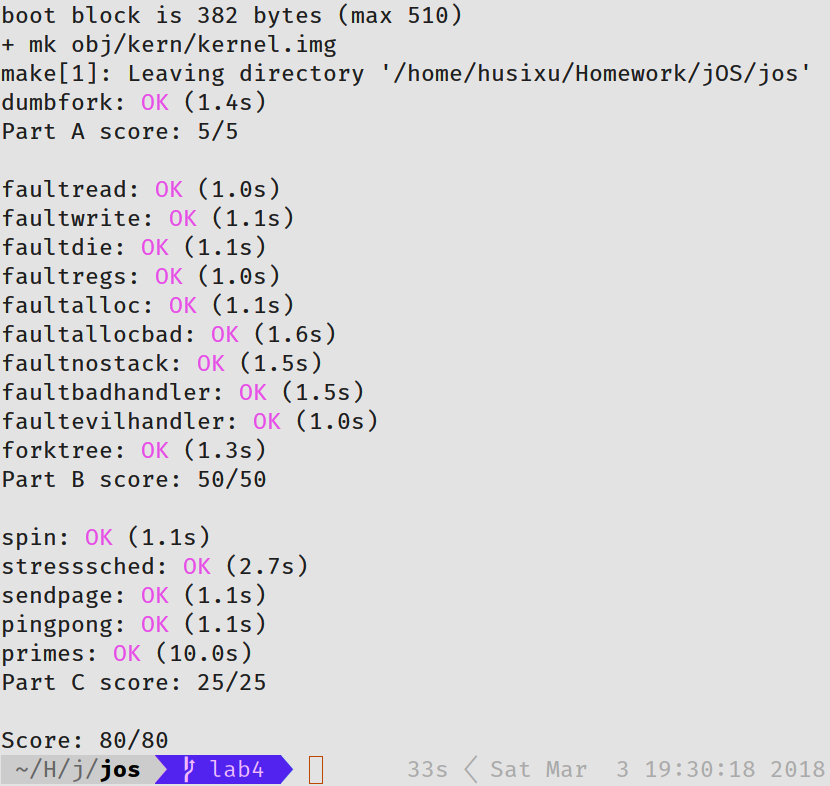
\includegraphics[width=0.65\linewidth]{lab4/exercise15_1.png}
    \caption{运行make grade输出结果}
    \label{fig:lab4/exercise15_1}
\end{figure}


